\documentclass{standalone}
\usepackage{tikz}
\usepackage{amsmath, amssymb}

\begin{document}
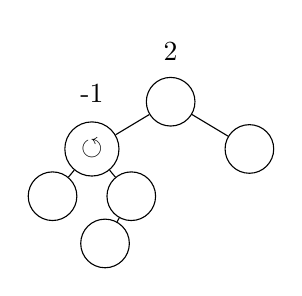
\begin{tikzpicture}[
  every node/.style={
    circle, draw, minimum width=6mm,
  }, 
  level/.style={
    sibling distance=20mm/#1,
    level distance=6mm
  }
  ]
  \node[label={2}] {\phantom{1}}
  child {
    node[label={-1}] {$\circlearrowleft$}
    child {
      node {\phantom{1}}
    }
    child {
      node {\phantom{1}}
      child {
        node {\phantom{1}}
      }
      child[missing]{}
    }
  }
  child {
    node {\phantom{1}}
  }
  ;
\end{tikzpicture}
\hspace{5mm} $\rightarrow$ \hspace{5mm}
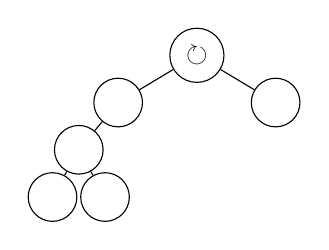
\begin{tikzpicture}[
  every node/.style={
    circle, draw, minimum width=6mm,
  }, 
  level/.style={
    sibling distance=20mm/#1,
    level distance=6mm
  }
  ]
  \node {$\circlearrowright$}
  child {
    node {\phantom{1}}
    child {
      node {\phantom{1}}
      child {
        node {\phantom{1}}
      }
      child {
        node {\phantom{1}}
      }
    }
    child[missing]{}
  }
  child {
    node {\phantom{1}}
  }
  ;
\end{tikzpicture}
\hspace{5mm} $\rightarrow$ \hspace{5mm}
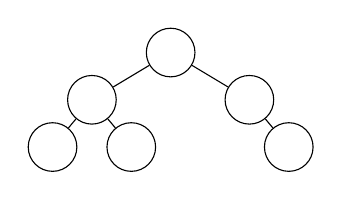
\begin{tikzpicture}[
  every node/.style={
    circle, draw, minimum width=6mm,
  }, 
  level/.style={
    sibling distance=20mm/#1,
    level distance=6mm
  }
  ]
  \node {\phantom{1}}
  child {
    node {\phantom{1}}
    child {node {\phantom{1}}}
    child {node {\phantom{1}}}
  }
  child {
    node {\phantom{1}}
    child[missing]{}
    child {node {\phantom{1}}}
  }
  ;
\end{tikzpicture}
\end{document}
